\documentclass[a4j]{jsarticle}
\usepackage{graphicx}
\usepackage{listings}

\title{2024年度プログラミング\textsc{iii} 演習課題}
\author{学籍番号: 35714121 \\ 氏名: 福富隆大}
\date{2024年11月14日}

\begin{document}
\maketitle

\textbf{1 はじめに} \\

本レポートは演習課題第7回の実行結果をまとめたものである。\\

\textbf{2 課題の実行結果} \\

\textmd{(課題7-1)} \\

課題の実行結果を図1に示す。 \\

\begin{figure}[htbp]
  \centering 
  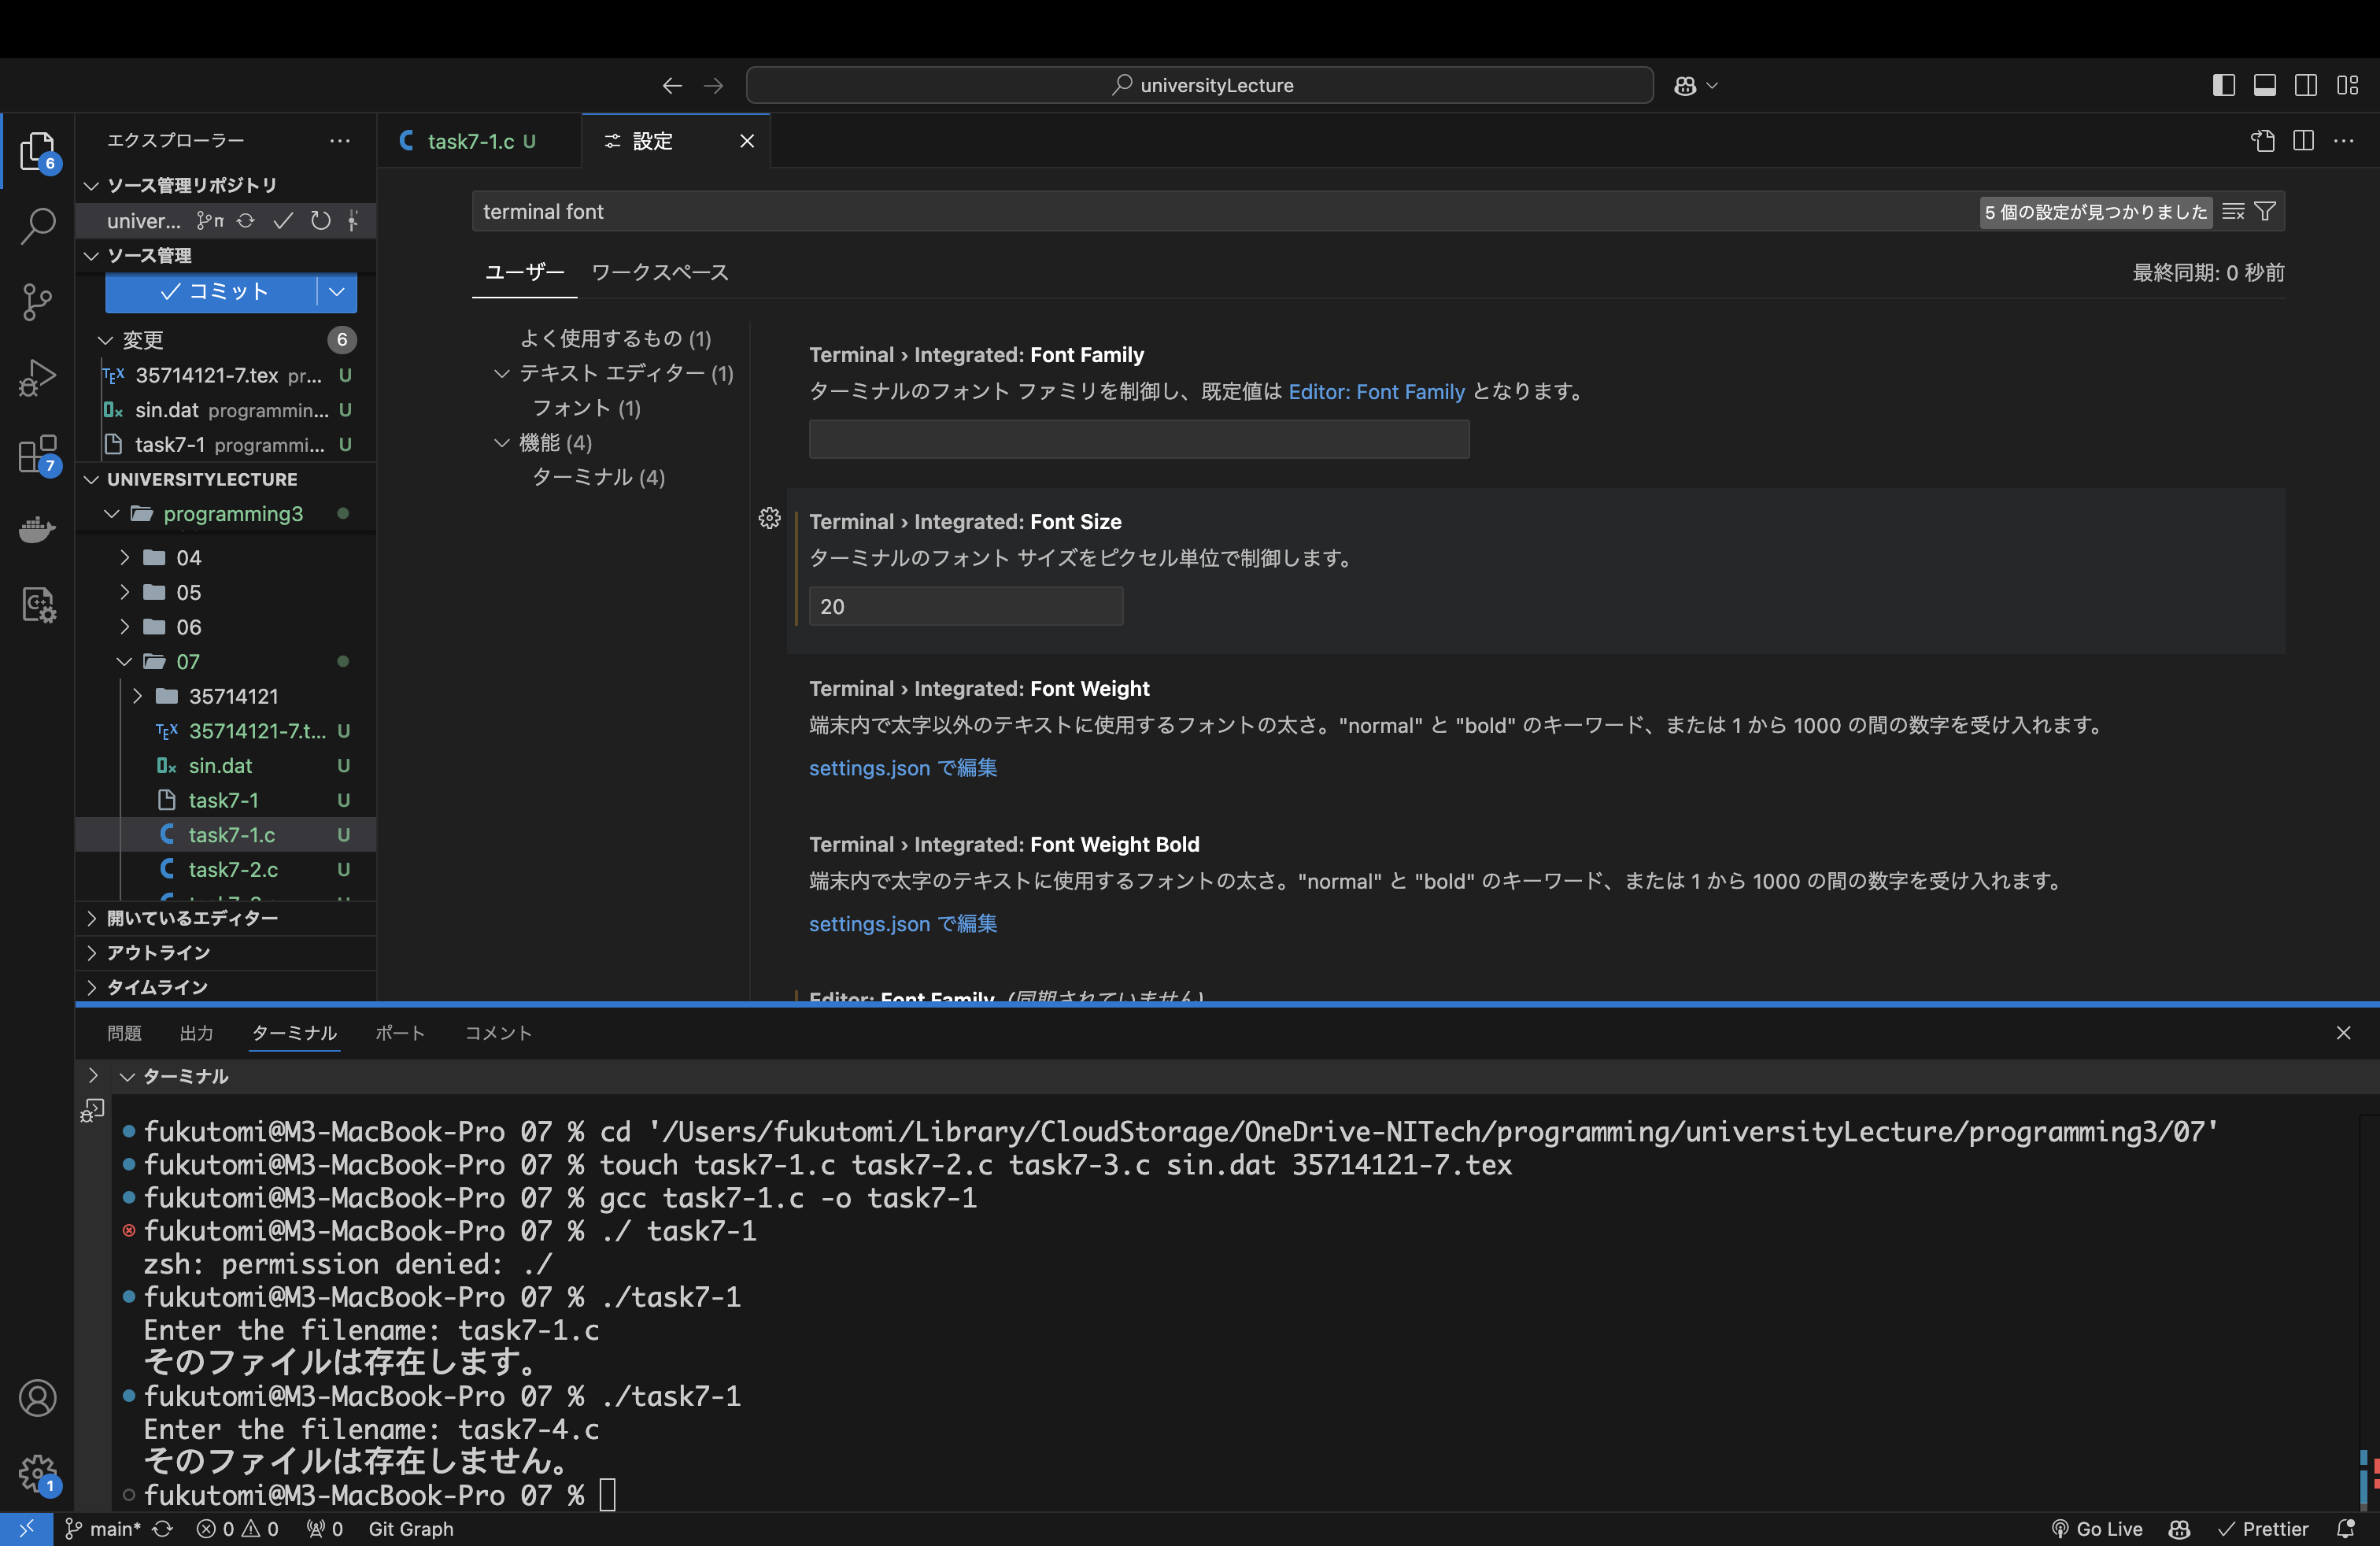
\includegraphics[width=10cm]{task7-1.eps}
  \caption{(ターミナルの部分に実行結果があります)}
  \label{fig:sample1} % ラベル名を変更
\end{figure}

\textmd{コードと結果の説明} 
スライドを参考にして、fileの名前を100文字を上限として読み込むプログラムを作った。\\
そして、ファイルを読み込みモードでファイルを読み込み、if文を使ってその名前のファイルが存在すれば『そのファイルは存在します。』と表示してファイルを閉じ、そうでなければ『そのファイルは存在しません。』と表示するプログラムを作成した。\\

\textmd{(課題7-2)} \\

課題の実行結果は課題7-3で示しているので省略。\\

\textmd{コードと結果の説明} \\
課題1と同じようにファイルを開き、if文でファイルが存在しなかったら、ファイルが存在しませんと表示し、ファイルが存在したら、ファイルにy=sin(2PIx)の値をx=0~x=1まで0.01刻みで書き込むプログラムを作成した。\\

\textmd{(課題7-3)} \\

課題の実行結果を図2に示す。 \\

\begin{figure}[htbp]
  \centering 
  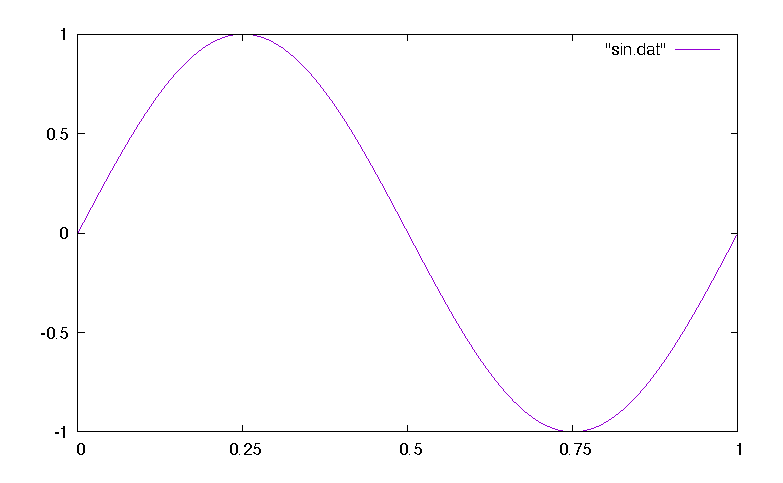
\includegraphics[width=10cm]{sin.eps}
  \label{fig:sample2} % ラベル名を変更
\end{figure}

\textmd{gnuplotコマンドの説明} 

gnuplotコマンドを使って、sin.datのデータをプロットし、x軸の目盛りを0から1まで0.25刻み、y軸の目盛りを-1から1まで0.5刻みに設定し、データを線で表示するように設定した。\\  
その後、ターミナルに出力された図をeps形式で出力し、sin.epsという名前で保存した。\\

\begin{lstlisting}[basicstyle=\ttfamily\footnotesize, frame=single]
% gnuplot <Enter>
gnuplot> plot "sin.dat"
gnuplot> set xtics 0, 1, 0.25
gnuplot> set ytics -1, 1, 0.5
gnuplot> set style data line
gnuplot> replot
gnuplot> set term eps
gnuplot> set output "sin.eps"
gnuplot> replot
gnuplot> set output
gnuplot> exit
\end{lstlisting}

\end{document}
